\documentclass{article}
\usepackage{enumitem}
\usepackage{graphicx}

\title{CS7033 Realtime Animationl \\ Lab 3 - Animation Hierarchy}
\author{Michael Stroughair \\Student Number: 12302190}

\usepackage{hyperref}
\hypersetup{
    colorlinks=true,
    linkcolor=blue,
    filecolor=magenta,      
    urlcolor=cyan,
}
 
\urlstyle{same}

\usepackage{listings}
\usepackage{color}
\usepackage{float} %required for the placement specifier H

\definecolor{dkgreen}{rgb}{0,0.6,0}
\definecolor{gray}{rgb}{0.5,0.5,0.5}
\definecolor{mauve}{rgb}{0.58,0,0.82}

\lstset{frame=tb,
  language=Java,
  aboveskip=3mm,
  belowskip=3mm,
  showstringspaces=false,
  columns=flexible,
  basicstyle={\small\ttfamily},
  numbers=none,
  numberstyle=\tiny\color{gray},
  keywordstyle=\color{blue},
  commentstyle=\color{dkgreen},
  stringstyle=\color{mauve},
  breaklines=true,
  breakatwhitespace=true,
  tabsize=3
}

\graphicspath{{images/}}

\begin{document}
\maketitle

\section{Examination}

\subsection{Correct Structure (~30\%)}

My code is made up of a Bone Class and a Skeleton class (which I renamed to the Hand Class, as it creates a hand model). The Hand class contains a number of pointers to Bones, represented first in a simple array, and then each finger on the hand has its own separate array, so that fingers can be accessed separately.

Each Bone has its own matrices to work with, a rotation matrix and a local transformation matrix. The rotation is taken care of through the use of quaternions. When a Bone is drawn, it is passed the model matrix used to draw its parent, which it multiplies with its own matrices to get its new location. That new global matrix is then passed to any children that Bone might have.

\begin{lstlisting}[language=Java]
void Bone::drawBone(mat4 projection, mat4 view, mat4 modelGlobal, GLuint shaderID, EulerCamera cam)
{
	mat4 modelLocal = modelGlobal * localTransform * rotMatrix;

	// light properties
	vec3 Ls = vec3(0.0001f, 0.0001f, 0.0001f);	//Specular Reflected Light
	vec3 Ld = vec3(0.5f, 0.5f, 0.5f);	//Diffuse Surface Reflectance
	vec3 La = vec3(1.0f, 1.0f, 1.0f);	//Ambient Reflected Light
	vec3 light = vec3(5, 10, -5.0f);//light source location
	vec3 coneDirection = light + vec3(0.0f, -1.0f, 0.0f);
	float coneAngle = 10.0f;
	// object colour
	vec3 Ks = vec3(0.1f, 0.1f, 0.1f); // specular reflectance
	vec3 Kd = BLUE;
	vec3 Ka = BLUE; // ambient reflectance
	float specular_exponent = 0.000000005f; //specular exponent - size of the specular elements

	drawObjectDebug(shaderID, view, projection, modelLocal, light, Ls, La, Ld, Ks, Kd, Ka, specular_exponent, cam, mesh, coneAngle, coneDirection, GL_TRIANGLES);
	
	
	for (GLuint i = 0; i < this->children.size(); i++)
	{
		this->children[i]->drawBone(projection, view, modelLocal, shaderID, cam);
	}
}
\end{lstlisting}

\subsection{Basic model showing a parent/child relationship (~10\%)}

I created a Hand that highlights the required relationship. The hand is made of the root, which I called palm, and then 5 fingers, each with 3 pieces representing it. All Bones with the exception of the palm are stored in two locations. The first location is the array that all the finger bones are stored in. The second is an array dedicated to that particular finger. This allows for operations to be performed on particular fingers, to every bone in the hand, or to a singular bone.

\subsection{Hand model (as described above) showing animation of the parent/child relationship (~40\%)}

The model itself is shown with a number of different animations. I first rotate the palm, and curl 4 of the fingers, to make the hand go from the default position (with the palm at the bottom and the fingers pointing in the positive y-axis) to a "thumbs up" position.

The next animation, shown when F1 is pressed, causes the palm to stop moving, and for all the fingers to curl inward, to form a fist.

The final two animations cause just the thumb to move, firstly with every bone curling up, and then secondly with just the first bone moving.

\subsection{Extra Features (~20\%}

\subsubsection{Good visual appearance of the hand (e.g., Using 3D model rather than Cylinders)}
My palm mesh was built in blender myself, but I chose to keep the basic cubes for the fingers.

\subsubsection{Forward Kinematics to create and interesting/plausible hand animation}

The functions that I call to make the hand move a quite basic, but essentially, the only thing I'm doing is applying a small rotation to one of the axis of the object each frame. This is achieved through my rotation functions, which each simply create a quaternion based on the added rotation, apply that rotation to the rotation matrix for the Bone, and then update the direction vectors. This allows me to create relatively interesting animations easily, which I spoke of in length above.

\begin{figure}[H]
\centering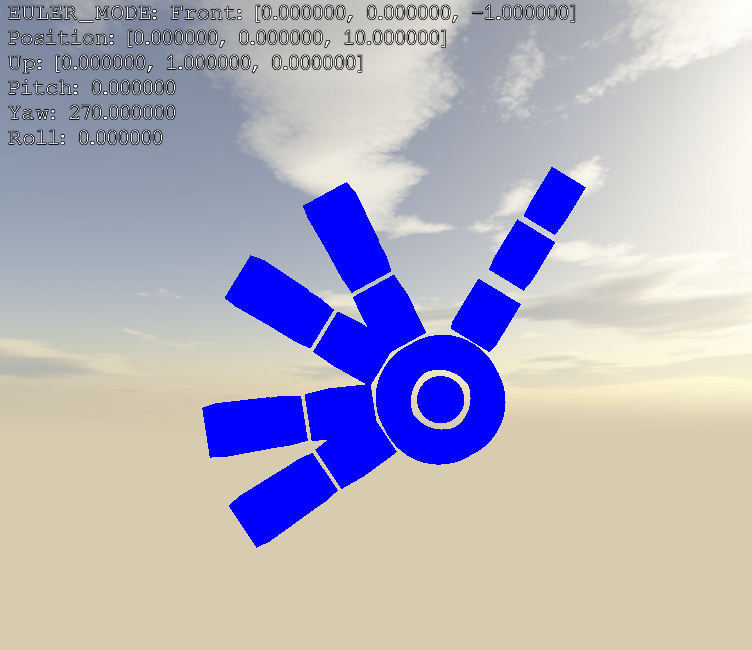
\includegraphics[scale=0.5]{scene.png}
\caption{\textit{Default parameter results}}
\end{figure}

\end{document}